\texttt{}\chapter{پیشینه پژوهش}

\section{مقدمه}
ظهور مدل‌های Transformer و انقلاب در یادگیری عمیق، یکی از تحولات اساسی در حوزه پردازش زبان طبیعی (NLP) و یادگیری ماشین به شمار می‌رود. این مدل‌ها باعث تغییرات عمده‌ای در نحوه ساخت و آموزش مدل‌های زبانی و همچنین در بسیاری از کاربردهای دیگر یادگیری ماشین شده‌اند. و توانستند بسیاری از مشکلات مدل های قبلی را حل کنند.

\section{مشکلات ترجمه ماشینی و ترانسفورمرها:}
در ابتدا، ترجمه ماشینی (MT) یک چالش اساسی در زمینه پردازش زبان طبیعی بود. مدل‌های اولیه‌ای مانند مدل‌های مبتنی بر قواعد (Rule-based models) برای ترجمه استفاده می‌شدند که در آن‌ها، ترجمه‌ها به صورت دستی با استفاده از قواعد زبانی مشخص تنظیم می‌شدند.
این روش‌ها هرچند دقیق بودند، اما محدودیت‌های زیادی داشتند و نمی‌توانستند ویژگی‌های پیچیده‌تر زبان را مدل‌سازی کنند.
سپس مدل‌های آماری (Statistical Models) معرفی شدند. این مدل‌ها از داده‌های ترجمه‌شده برای آموزش مدل‌های آماری استفاده می‌کردند که احتمال ترجمه‌ای صحیح را براساس شواهد آماری محاسبه می‌کردند. مدل‌هایی مانند مدل‌های ترجمه آماری مبتنی بر جمله (Phrase-based Statistical Models) از این نوع بودند، که قادر به ترجمه جملات بهتر از مدل‌های مبتنی بر قواعد بودند، اما هنوز هم در ترجمه‌های پیچیده با مشکلاتی روبه‌رو بودند.  بعد از این مدل ها مدل ها بازگشتی به وحود آمدند که مشکلات آن را در فصل گذشته بیان کردیم و د نهایت این مشکلات باعث به وجود آمدن ترانسفورمر ها شد.

\section{ظهور ترانسفورمر ها:}
در سال 2017 مقاله ... توسط گوگل منتشر شد که مفهوم جدیدی به نام ترانسفورمر ها را بیان کرد.
این مقاله به موضوع ترجمه ماشینی پرداخت و نشان داده با استفاده از مفهوم مکانیزم توجه (Attention-Mechanism) می توان بسیاری از مشکلات مدل های قبلی را حل کرد.
این مدل ها از پردازش موازی استفاده میکردند بر خلاف مدل های قبلی که از پردازش های سریالی استفاده میکردند. و این مدل ها قادر هستند به طور همزمان به تمام بخش های ورودی توجه کند.
و این کار باعث شد که ترانسفورمر ها در پردازش تصویر و متن بسیار سریع تر و دقیق تر از مدل های قبلی عمل کنند.


 \section{معماری ترانسفورمر ها:}
 
 در تصویر ... معماری ترانسفورمر نمایش داده شده است  و بخش هاو اجزای مختلف آن مشخص شده است که از دو بخش اصلی انکودر و دیکدر تشکیل شده است هدف انکودر این است که داده ورودی را میگیرد  و ویژگی های آن را استخراج میکند و هدف دیکدر این است که ویژگی های استخراج شده را به زبان مقصد تبدیل میکند. که به طور مختصر به معماری  و بخش های مختلف آن میپردازیم.
 
 \begin{figure}[h]
 	\centering
 	\begin{minipage}[b]{0.45\textwidth}
 		\centering
 		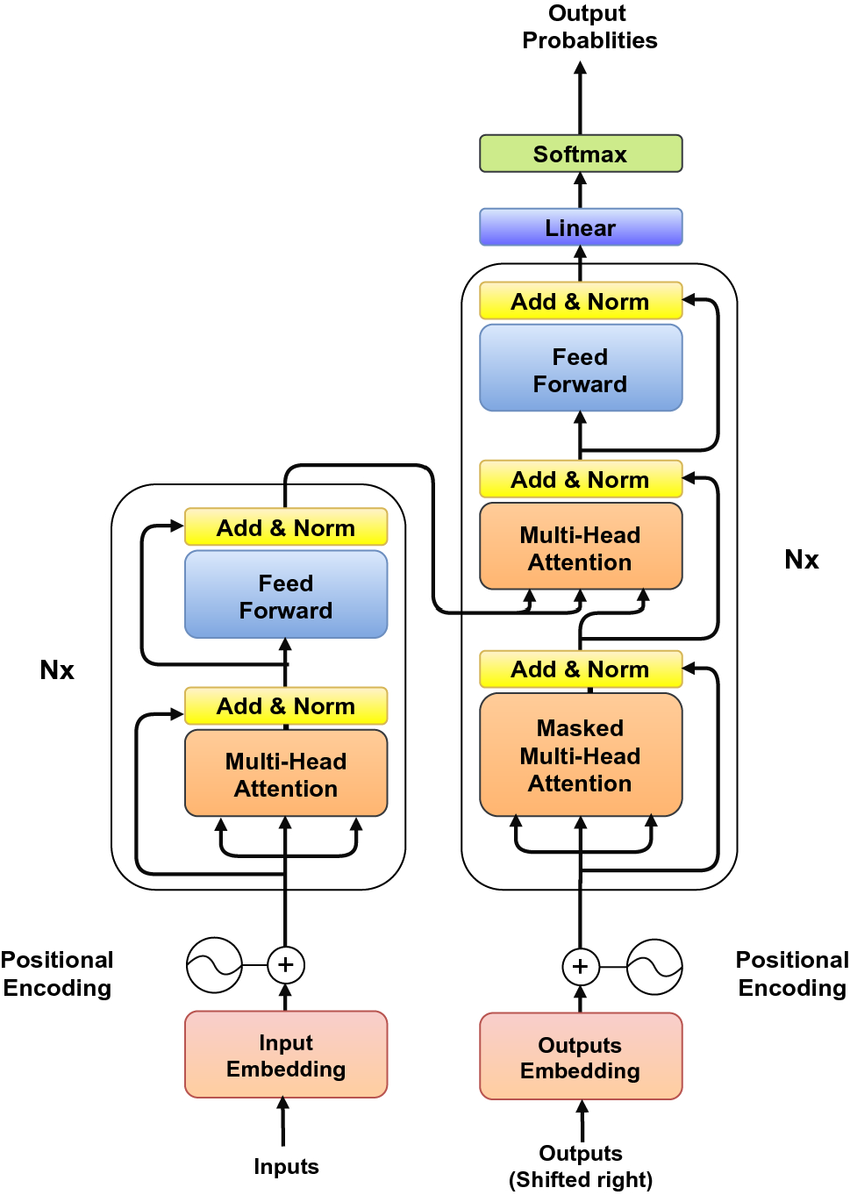
\includegraphics[width=\textwidth]{Transformer-model-architecture.png}
 		\caption{معماری ترانسفورمر ها}
 		\label{fig:transformer_architecture}
 	\end{minipage}
 	\hfill

 \end{figure}

\subsection{Embedding:}
در زبان طبیعی کلمات به شکل رشته های متنی هستند مانند کتاب ، ماشین و ... 
کامپیوتر ها نمیتوانند به طور مستقیم به شکل رشته های متنی این کلمات را پردازش کنند. 
به همین دلیل در یادگیری ماشین ما این کلمات را به شکل یک بردار نمایش می دهیم. و آن بردار بیانگر آن کلمه در مدل است تا ماشین بتواند آن کلمه را پردازش کند.

این بردار ها ویژگی های کلمه را فضای عددی نمایش میدهد. 
روش های مختلفی برای تبدیل متن به بردار وجود دارند.
از جمله این روشها میتوان به روش Word2Vec و GloVe  اشاره کرد.
همانطور که در تصویر ... نشان داده شده است، هر کلمه که به صورت توکن است ابتدا در دیکشنری تعریف شده پیدا می شود و پس از پیدا شدن در دیکشنری با استفاده از روش های embedding، هر کلمه به برداری از اعداد تبدیل می شوند.
این embedding  ها شباهت های معنایی بین کلمات را مدل سازی میکنند به طوری که کلماتی که از نظر معنایی شبیه به هم هستند، بردار آن ها نیز به یک دیگر نزدیک تر است. و به این ترتیب کلمات برای مدل ها و شبکه های عصبی قابل فهم می شود.



 \begin{figure}[h]
	\centering
	\begin{minipage}[b]{0.7\textwidth}
		\centering
		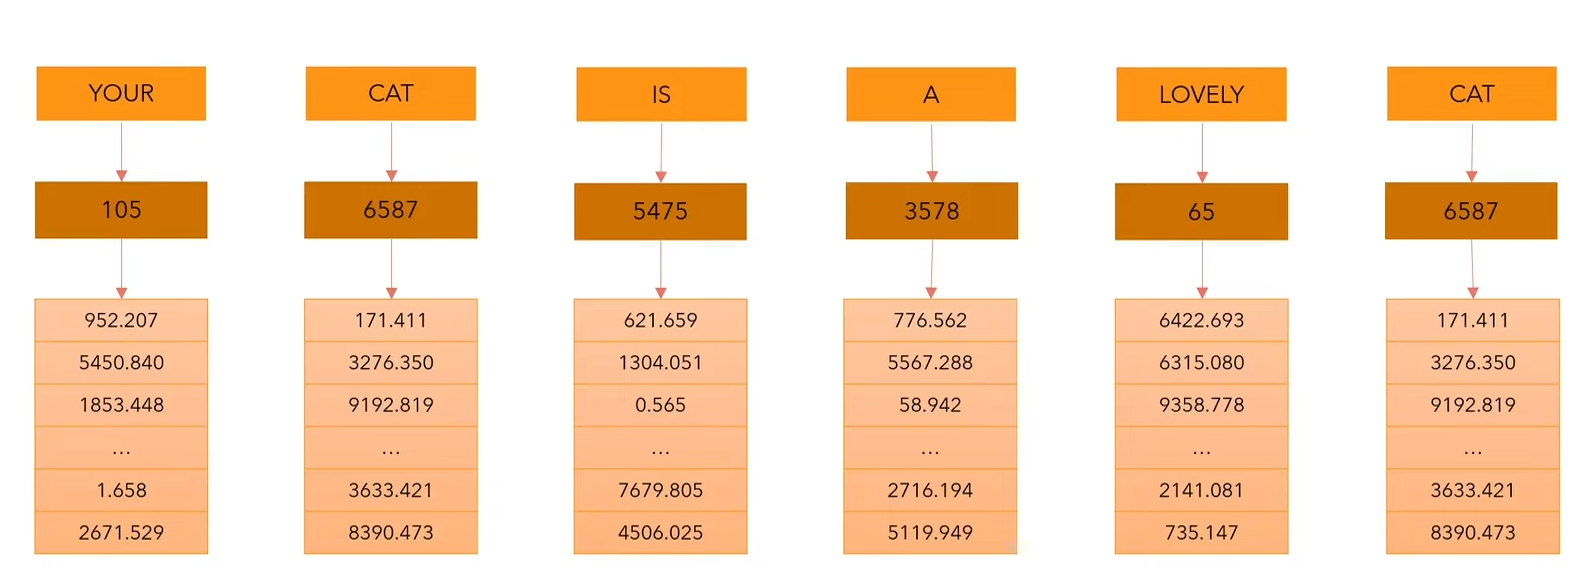
\includegraphics[width=\textwidth]{transformer_images/word_embedding.png}
		\caption{word embedding}
		\label{fig:word_embedding}
	\end{minipage}
	\hfill
	
\end{figure}



\subsection{positional embedding:}

ما تا الان هر کلمه را به برداری از اعداد که برای مدل قابل فهم باشد، تبدیل کرده ایم. 
اما مدل های ترانسفورمر نمیتوانند جایگاه هر کلمه را تشخیص دهند. در مدل های ترانسفومر بر خلاف مدل های بازگشتی  به دلیل این که کلمه های به صورت موازی وارد میشوند نیاز داریم تا جایگاه هر کلمه را بدانیم به طور مثال جمله من تو رو دوست داریم باید به طور دقیق بدانیم کلمه من، کلمه اول حمله است، کلمه تو کلمه دوم جمله است و ...
حال ما باید به مدل توالی این کلمات را بفهمیم، پس ما نیاز داریم به مدل یک سری اطلاعات اضافی بدهیم به طوری که مدل توالی کلمات را یاد بگیرد. روش های مختلفی برای اضافه کردن positional embedding  به مدل وجود دارد که در ترانسفومرر ها از روش Sinusoidal Positional Embedding استفاده میشود.
این روش قابل یادگیری نیست و صرفا از یک سری فرمول های ساده برای positional embedding  استفاده میکند.

برای موقعیت \( pos \) در توالی و بعد \( i \) در فضای برداری، تعبیه موقعیتی به صورت زیر تعریف می‌شود:

\[
PE(pos, 2i) = \sin\left( \frac{pos}{10000^{\frac{2i}{d}}} \right)
\]

و برای مقادیر فرد:

\[
PE(pos, 2i+1) = \cos\left( \frac{pos}{10000^{\frac{2i}{d}}} \right)
\]







\begin{figure}[h]
	\centering
	\begin{minipage}[b]{0.7\textwidth}
		\centering
		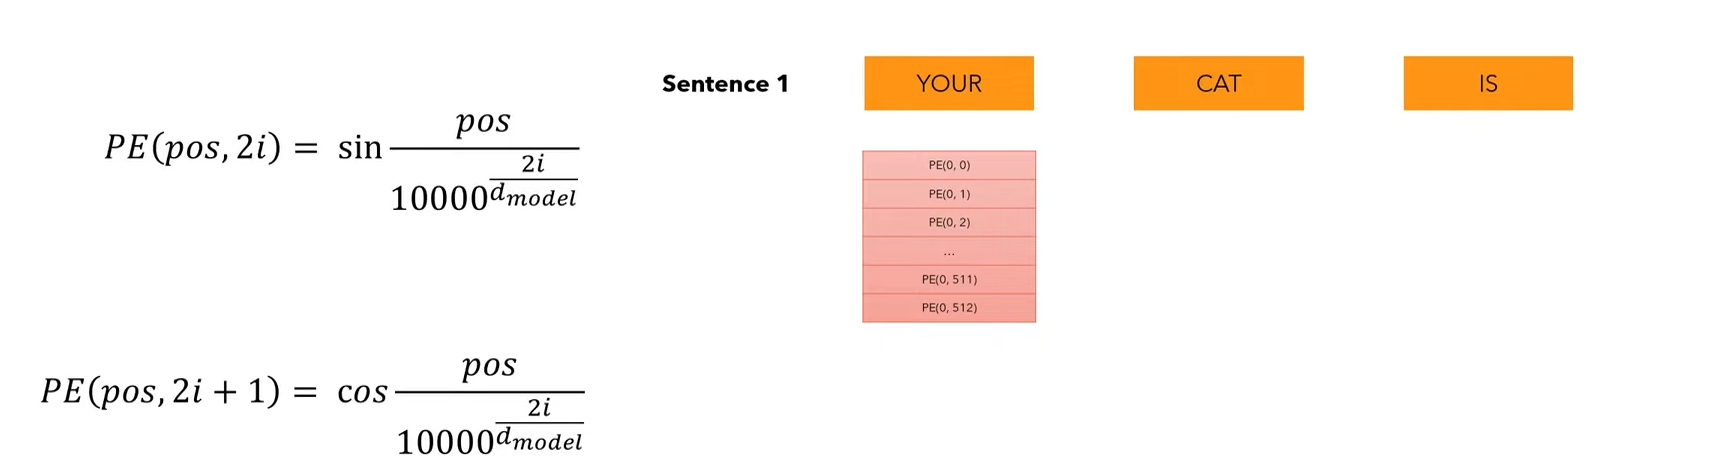
\includegraphics[width=\textwidth]{transformer_images/positional_embedding_formula .png}
		\caption{word embedding}
		\label{fig:positional embedding}
	\end{minipage}
	\hfill
	
\end{figure}





- \( pos \): موقعیت کلمه در توالی است. برای مثال، اگر توالی ورودی شامل \( N \) کلمه باشد، موقعیت‌ها از \( 0 \) تا \( N-1 \) تغییر می‌کنند. به عبارت دیگر، \( pos \) می‌تواند هر عددی از مجموعه \( \{0, 1, 2, \dots, N-1\} \) باشد که نشان‌دهنده موقعیت یک کلمه خاص در توالی است.

- \( i \): شاخص بعد در بردار موقعیتی است. این متغیر به اندیس بعدی که موقعیت کلمه در آن نمایش داده می‌شود اشاره دارد. برای مثال، اگر فضای برداری مدل دارای ابعاد \( d \) باشد، \( i \) از \( 0 \) تا \( d-1 \) تغییر می‌کند.

- \( d \): ابعاد فضای برداری مدل است. این مقدار مشخص می‌کند که هر کلمه در توالی به چه تعداد ابعاد در فضای برداری نگاشت می‌شود. به عبارت دیگر، \( d \) نشان‌دهنده تعداد ویژگی‌ها (یا ابعاد) در بردار موقعیتی است.

- \( 10000 \): یک مقدار ثابت است که برای تنظیم مقیاس توابع تناوبی استفاده می‌شود. این مقدار به‌گونه‌ای تنظیم شده است که از نوسانات زیاد جلوگیری کند و همچنین فرکانس‌های مختلفی را برای ابعاد مختلف به وجود آورد.

همانطور که در شکل زیر مشاهده میکنید بعد از embedding  کلمات  positional embedding  به آن اضافه می شود.
که در این روش از توابع سینوس و کسینوس استفاده میشود.
این توابع موقعیت ها را در فضای برداری به گونه ای نگاشت میکنند که مدل بتواند از ترتیب کلمات در توالی آگاه باشد.این ویژگی به مدل کمک میکند تا مدل توالی زمانی را بتواند درک کند و الگو های زمانی را شبیه سازی کند.
از مزایای این مدل میتوان به عدم نیاز به آموزش و توزیع متوازن جایگاه هر کدام از کلمات اشاره کرد.


\begin{figure}[h]
	\centering
	\begin{minipage}[b]{0.7\textwidth}
		\centering
		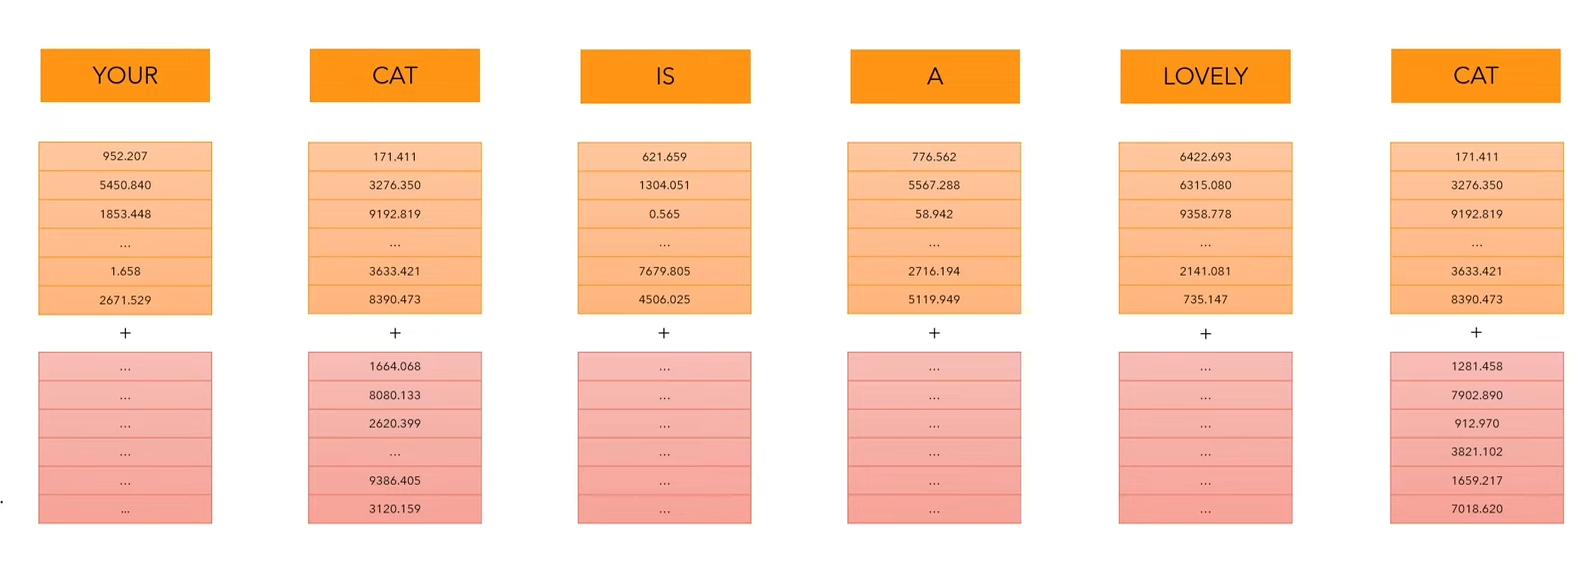
\includegraphics[width=\textwidth]{transformer_images/positional_embedding.png}
		\caption{word embedding}
		\label{fig:word embedding + positional embedding}
	\end{minipage}
	\hfill
	
\end{figure}






\subsection{attention:}



در روش‌های قدیمی (مانند RNN یا lstm)، توالی ورودی (مثلاً یک جمله) معمولاً به‌صورت گام‌به‌گام پردازش می‌شد. اما در ترانسفورمر می‌خواهیم مدلی داشته باشیم که به هر موقعیت (مثلاً یک کلمه) در توالی نگاه کند و به همهٔ موقعیت‌های دیگر نیز به‌صورت موازی دسترسی داشته باشد. به این مفهوم \textbf{توجه} می‌گوییم.
م
به زبان ساده، وقتی توکن (کلمه) $i$ به توکن‌های دیگر نگاه می‌کند، می‌خواهد بداند کدام توکن‌ها برای تفسیر معنای خودش مهم‌ترند.

به طور مثال در جمله  یک گربه روی زمین نشسته است میخواده بداند کلمه گربه به واژه نشستن بیشتر توجه کند یا به زمین، مثلا در این جا فعل نشستن ارتباط نزدیک تری به گربه دارد، و از نظر معنایی مرتبط تر است.




\[
Q = \text{Query (پرسش)}, \quad K = \text{Key (کلید)}, \quad V = \text{Value (مقدار / ارزش)}
\]

در \textbf{Scaled Dot-Product Attention}، ابتدا شباهت یا ارتباط بین \textit{Query} و \textit{Key} را با محاسبهٔ ضرب داخلی (Dot Product) به‌دست می‌آوریم، سپس آن را نرمال می‌کنیم (با تقسیم بر \( d_k \)) و از تابع \textit{softmax} استفاده می‌کنیم تا ضرایب توجه (Attention Weights) را به‌دست آوریم. در نهایت با همین ضرایب، ترکیبی خطی از بردارهای \textit{Value} را می‌گیریم.

فرمول به‌شکل زیر است:

\[
\text{Attention}(Q, K, V) = \text{softmax}\left( \frac{QK^T}{\sqrt{d_k}} \right) V
\]

که در آن:

\[
Q \in \mathbb{R}^{n \times d_k} \quad \text{ماتریس پرسش برای} \, n \, \text{توکن}
\]
\[
K \in \mathbb{R}^{n \times d_k} \quad \text{ماتریس کلید برای} \, n \, \text{توکن}
\]
\[
V \in \mathbb{R}^{n \times d_v} \quad \text{ماتریس مقدار برای} \, n \, \text{توکن}
\]

\[
d_k \quad \text{ابعاد بردارهای پرسش و کلید است (معمولاً} \, d_k = d_{\text{model}} \, \text{در حالت چندسری)}
\]

تقسیم بر \( d_k \) باعث می‌شود مقدار ضرب داخلی در ابعاد بالا خیلی بزرگ نشود و شیب‌ها (Gradients) پایدار بمانند.

\[
\alpha = \text{softmax}\left( \frac{QK^T}{\sqrt{d_k}} \right)
\]
\(\alpha\) یک ماتریس با ابعاد \( n \times n \) است که سطر \( i \)-ام آن ضرایب توجه برای توکن \( i \) را نشان می‌دهد.

تفسیر ضرایب توجه: هر سطر از \( \alpha \) نشان می‌دهد که توکن فعلی به چه توکن‌هایی در جمله، با چه شدتی توجه می‌کند.



\begin{figure}[h]
	\centering
	\begin{minipage}[b]{0.7\textwidth}
		\centering
		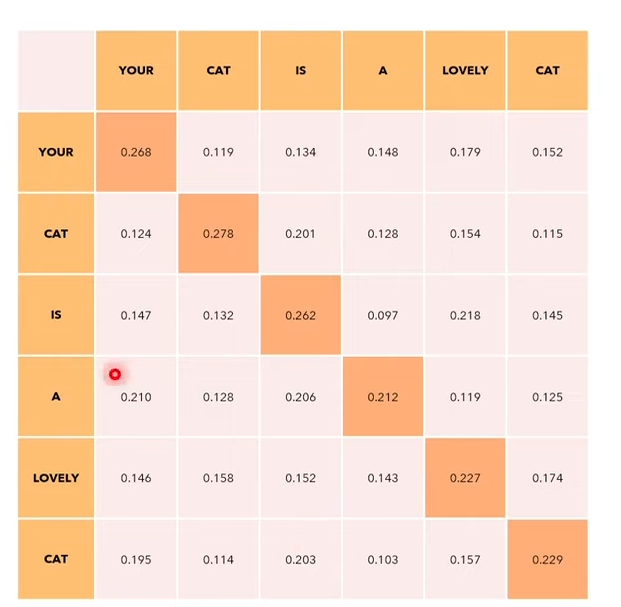
\includegraphics[width=\textwidth]{transformer_images/attention.png}
		\caption{Attention}
		\label{fig:attention}
	\end{minipage}
	\hfill
	
\end{figure}





ایدهٔ چندسری:  
به‌جای آنکه فقط یک‌بار \( Q, K, V \) بسازیم و عملیات توجه را انجام دهیم، چندین مجموعهٔ متفاوت \( Q_i, K_i, V_i \) می‌سازیم (هر کدام یک «Head» یا سر نام دارد) و به‌صورت موازی محاسبات Attention را انجام می‌دهیم. سپس خروجی همهٔ این Headها را کنار هم قرار داده (Concat) و در نهایت با یک ماتریس وزن دیگر ضرب می‌کنیم تا به بعد اصلی بازگردیم.

فرمول مربوط به این ایده به‌شکل زیر است:

\[
\text{head}_i = \text{Attention}(Q_i, K_i, V_i)
\]
\[
\text{MultiHead}(Q, K, V) = [\text{head}_1 \oplus \cdots \oplus \text{head}_h] W_O
\]

که در آن \( \oplus \) نشان‌دهندهٔ عمل الحاق (Concatenation) است.

ماتریس وزن \( W_O \) به‌شکل زیر است:

\[
W_O \in \mathbb{R}^{(h \cdot d_v) \times d_{\text{model}}}
\]

که \( W_O \) ماتریسی است که خروجی الحاق‌شده را به بعد \( d_{\text{model}} \) برمی‌گرداند.





\begin{figure}[h]
	\centering
	\begin{minipage}[b]{0.9\textwidth}
		\centering
		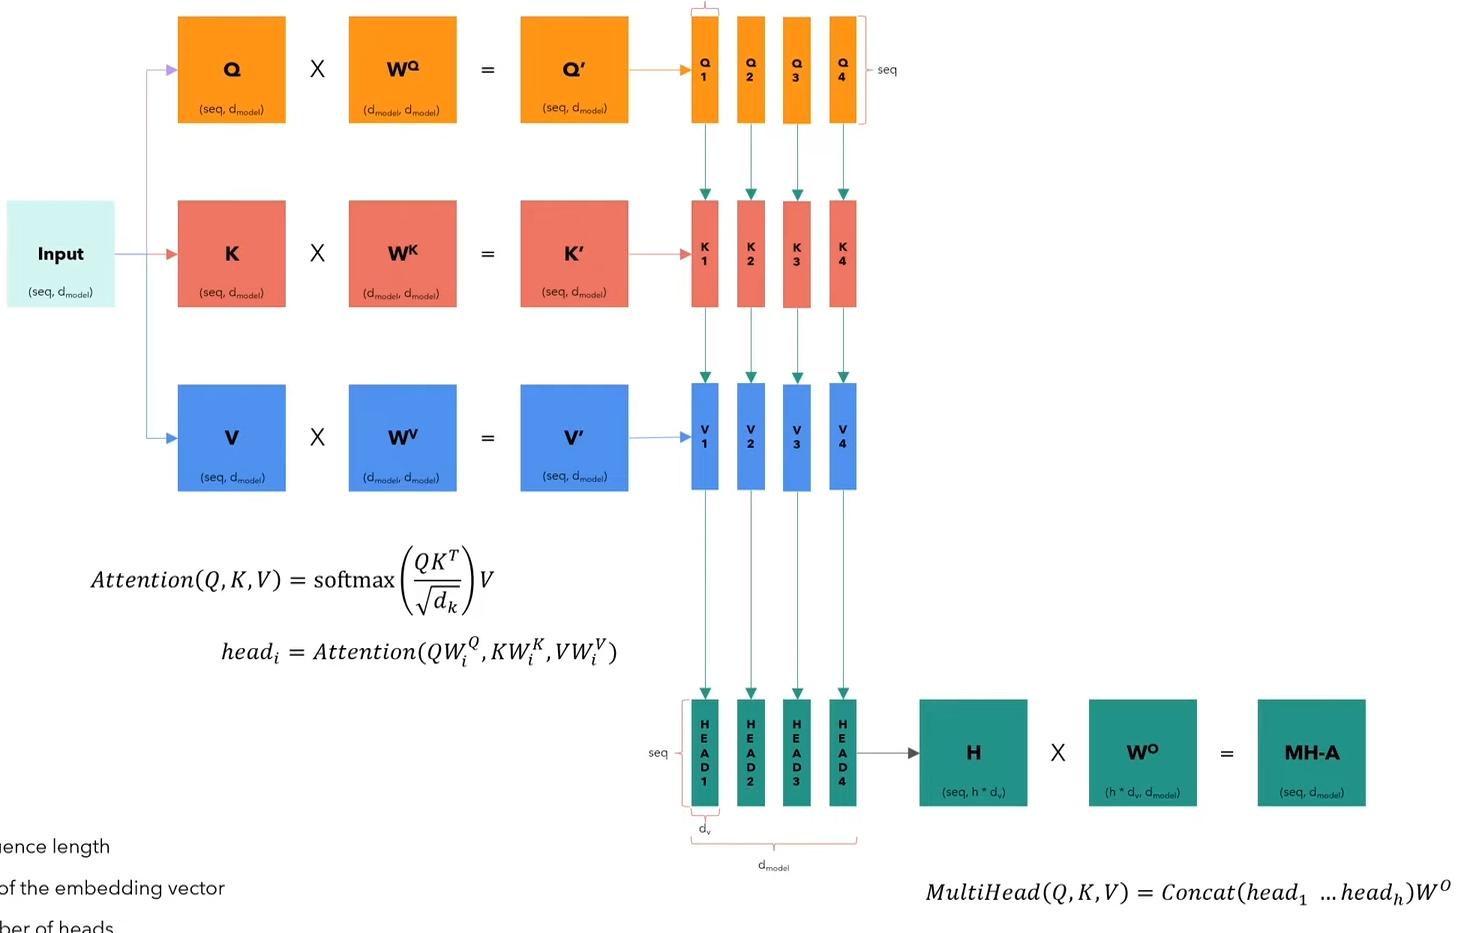
\includegraphics[width=\textwidth]{transformer_images/multi_head_attention.png}
		\caption{multi head attention}
		\label{fig:attention}
	\end{minipage}
	\hfill
	
\end{figure}



\subsection*{چرا چندین سر؟}

\textbf{مشاهدهٔ چند منظر متفاوت:} هر Head می‌تواند الگوهای گوناگونی از وابستگی‌ها را بیاموزد (مثلاً یک Head می‌تواند یاد بگیرد کلمهٔ فعلی با کلمات همسایهٔ نزدیک خود بیشتر مرتبط شود، یک Head دیگر روی ارتباط با کلماتی در فاصلهٔ دورتری متمرکز باشد، Head دیگر روی مطابقت جنس و تعداد در دستور زبان و ...).

\textbf{افزایش ظرفیت مدل:} با داشتن چند Head، مدل می‌تواند قدرت بیان بیشتری داشته باشد.

\textbf{ابعاد کمتر در هر Head:} در عمل، اگر \( d_{\text{model}} \) مثلاً 512 باشد، و تعداد Headها \( h = 8 \)، آنگاه هر Head ابعادی در حدود \( d_k = 64 \) خواهد داشت؛ و این محاسبات ضرب داخلی را نیز مقیاس‌پذیر و قابل موازی‌سازی می‌کند.


\subsection{Residual Connection (Add):}
در معماری های های مختلف هنگامی که تعداد لایه ها زیاد  میشود، اغلب دچار ناپایداری گرادیان (Vanishing/Exploding Gradients) میشوند. و باعث مشکل در آموزش مدل میشود.
در مدل ترانسفورمر به جای این که خروجی attention  را به صورت مستقیم به لایه بعدی بدهیم، ورودی آن را نیز حفظ کرده و به خروجی اضافه میکنیم.
اگر \( x \) ورودی به زیرماژول و \( \text{SubLayer}(x) \) خروجی آن زیرماژول باشد، در انتهای کار، ما عبارت زیر را محاسبه می‌کنیم:


\[
x + \text{SubLayer}(x)
\]

این جمع به صورت عنصر به عنصر (Element-wise Addition)  انجام میشود.


\subsection{مزایای Residual Connection در ترانسفورمر}

\subsection*{کمک به جریان یافتن گرادیان}

وقتی ورودی مستقیماً به خروجی اضافه می‌شود، مسیری مستقیم برای عبور شیب (گرادیان) به عقب ایجاد می‌گردد.
در صورت نبود این اتصال، اگر شبکه عمیق شود، گرادیان‌ها ممکن است در لایه‌های پایین محو شوندو عملا gradient vanishing رخ میدهد.

\subsection*{حفظ اطلاعات اصلی (هویت ورودی)}

حتی اگر زیرماژول تغییری در اطلاعات ورودی ایجاد کند، با وجود Residual Connection، ورودی اصلی همواره در خروجی نهایی حضور دارد.
این ویژگی باعث می‌شود در صورت ناکافی بودن یادگیری زیرماژول یا در مراحل اولیهٔ آموزش، دست‌کم بخشی از سیگنال/اطلاعات خام به لایه‌های بالاتر برسد.

\subsection*{کاهش ریسک تخریب ویژگی‌ها}

در شبکه‌های عمیق، یکی از مشکلات این است که هر لایه ممکن است بخشی از اطلاعات مفید را تخریب کند. Residual Connection تضمین می‌کند که اگر لایه‌ای به هر دلیل نتوانست الگوی بهینه را یاد بگیرد، اطلاعات قبلی حداقل به صورت دست‌نخورده تا حدی منتقل می‌شود.

\section{Layer Normalization (Norm):}

در یادگیری عمیق، نرمال‌سازی (Normalization) داده‌های یک لایه یا فعال‌سازی‌ها، اغلب به سرعت بخشیدن به همگرایی و پایدار کردن آموزش کمک شایانی می‌کند. شاید معروف‌ترین نوع نرمال‌سازی، \textbf{Batch Normalization} باشد که پیش‌تر در کارهای بینایی (CNNها) بسیار مورداستفاده قرار گرفت.

\textbf{Layer Normalization} روشی جایگزین است که در ترانسفورمر استفاده می‌شود. علت اصلی این انتخاب، ماهیت توالی‌محور (Sequence) بودن داده‌ها در NLP و عدم تمایل به وابستگی به آمار مینی‌بچ است.



\subsection*{تفاوت Layer Norm با Batch Norm}

\subsection*{Batch Normalization:}

در Batch Norm، برای نرمال‌سازی، میانگین و واریانس روی تمام نمونه‌های موجود در مینی‌بچ (و نیز در طول ابعاد ویژگی) محاسبه می‌شود.
این موضوع در NLP کمی دردسرساز است؛ چون ترتیب (Order) توکن‌ها، طول جمله‌ها و حتی اندازهٔ مینی‌بچ ممکن است نامنظم باشد.
همچنین به خاطر تنوع طول توالی‌ها (Sequence Length)، پیاده‌سازی Batch Norm می‌تواند پیچیده شود.

\subsection*{Layer Normalization:}

در Layer Norm، برای هر توکن به‌صورت جداگانه (در طول بُعد ویژگی)، میانگین و واریانس گرفته می‌شود.
فرض کنید در یک لایه، بردار \( h_i \in \mathbb{R}^{d_{\text{model}}} \) مربوط به توکن \( i \) باشد؛ یعنی ابعاد ویژگی آن \( d_{\text{model}} \) است. ما میانگین \( \mu_i \) و واریانس \( \sigma_i^2 \) را از اجزای این بردار محاسبه می‌کنیم:

\[
\mu_i = \frac{1}{d_{\text{model}}} \sum_{k=1}^{d_{\text{model}}} h_{i,k}, \quad
\sigma_i^2 = \frac{1}{d_{\text{model}}} \sum_{k=1}^{d_{\text{model}}} (h_{i,k} - \mu_i)^2
\]

سپس نرمال‌سازی برای هر مؤلفهٔ \( k \) در بردار توکن \( i \) به شکل زیر انجام می‌شود:

\[
\hat{h}_{i,k} = \frac{h_{i,k} - \mu_i}{\sqrt{\sigma_i^2 + \epsilon}}
\]

در نهایت، برای این‌که مدل بتواند مقیاس و بایاس جدیدی یاد بگیرد، شبیه Batch Norm، دو پارامتر \( \gamma \) (Scale) و \( \beta \) (Bias) نیز در طول بعد ویژگی اعمال می‌شوند:

\[
\text{LayerNorm}(h_i) = \gamma \odot \hat{h}_i + \beta
\]

که در آن \( \gamma, \beta \in \mathbb{R}^{d_{\text{model}}} \) هستند و \( \odot \) ضرب عنصر به عنصر است.

\subsection*{مزایای Layer Normalization در ترانسفورمر}

\begin{itemize}
	\item \textbf{بی‌نیازی از وابستگی به ابعاد مینی‌بچ:}  
	با Layer Norm، می‌توان حتی با اندازهٔ مینی‌بچ برابر ۱ نیز به‌خوبی آموزش دید، چراکه آمارها وابسته به ابعاد ویژگی‌اند و نه مینی‌بچ.
	
	\item \textbf{پایدارسازی توزیع فعال‌سازی‌ها:}  
	زمانی که مدل در حال یادگیری است، توزیع‌های داخلی لایه‌های میانی ممکن است تغییر کند (پدیدهٔ Internal Covariate Shift). Layer Norm با نرمال‌سازی این توزیع، آموزش را پایدارتر و سریع‌تر می‌کند.
	
	\item \textbf{سازگاری با داده‌های توالی‌محور:}  
	هر توکن را جداگانه نرمال می‌کند و نگرانی‌ای بابت ترتیب طول جمله‌ها، یا قرار گرفتن چند جملهٔ کوتاه/بلند در یک مینی‌بچ نداریم.
\end{itemize}





در معماری ترانسفورمر، پس از خروجیِ هر زیرماژول (مثل Attention یا MLP)، مراحل به‌شکل زیر است:

\textbf{Residual Connection:} ابتدا ورودی همان زیرماژول (مثلاً بردار \( x \)) را با خروجی زیرماژول (\( \text{SubLayer}(x) \)) جمع می‌کنیم. حاصل این جمع را می‌توان چنین نوشت:

\[
z = x + \text{SubLayer}(x)
\]

این \( z \) حالا ترکیبی از اطلاعات اصلی ورودی و اطلاعات یادگرفته‌شده توسط SubLayer است.

\textbf{Layer Normalization:} سپس این بردار \( z \) را وارد لایهٔ \text{LayerNorm} می‌کنیم:

\[
y = \text{LayerNorm}(z)
\]

خروجی نهایی را می‌توان به لایهٔ بعدی پاس داد یا به مرحلهٔ بعدی در همین لایه.

به‌عبارتی اگر بخواهیم در یک فرمول واحد بیان کنیم:

\[
\text{Add \& Norm} = \text{LayerNorm}\left(x + \text{SubLayer}(x)\right)
\]

\section{decoder:}

دیکودر  در معماری ترانسفورمرها وظیفه تولید خروجی نهایی را بر عهده دارد. این خروجی معمولاً می‌تواند توالی هدف (Target Sequence) باشد، مثل ترجمه یک جمله یا پیش‌بینی توکن‌های بعدی در یک توالی.
در ابن بخش دیکدر دو ورودی اصلی دارد:
 توالی هدف که معمولاً به صورت خودکار تولید می‌شود (مثلاً در ترجمه ماشینی یا تولید متن)، و نمایش (Representation) کدشده که توسط انکودر (Encoder) تولید شده است و شامل ویژگی‌های استخراج‌شده از توالی ورودی می‌باشد. دیکودر از این ورودی‌ها استفاده می‌کند تا به صورت گام‌به‌گام، خروجی نهایی خود را تولید کند.
 
 
 همانطور که در تصویر مشاهده میکنید دیکدر دو ورودی دارد.
 

\begin{figure}[h]
	\centering
	\begin{minipage}[b]{0.25\textwidth}
		\centering
		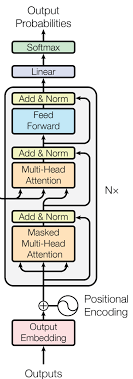
\includegraphics[width=\textwidth]{transformer_images/decoder.png}
		\caption{Decoder}
		\label{fig:Decoder}
	\end{minipage}
	\hfill
	
\end{figure}

تمامی بخش های دیکدر مانند انکدر میباشند اما در دیکدر masked multi head attention  وجود دارد.

\section{masked multi head attention}


در ترانسفورمر، مکانیزم Multi-Head Attention در بخش دیکودر به‌صورت Masked پیاده‌سازی می‌شود تا مدل نتواند توکن‌های آینده را ببیند و به‌صورت خودبازگشتی (Autoregressive) توکن بعدی را پیش‌بینی کند.
در واقع ایده اصلی استفاده از mask  جلوگیری از مشاهده آینده است.




 در معماری‌های خودبازگشتی (\textit{Autoregressive})، مدل در گام \( i \) از دیکودر تنها باید به توکن‌های قبلی \( \{ y_1, \dots, y_{i-1} \} \) دسترسی داشته باشد؛ اما نه به توکن‌های \( \{ y_{i+1}, y_{i+2}, \dots \} \). اگر مدل بتواند توکن‌های آینده را «نگاه» کند، پیش‌بینی توکن بعدی آسان و غیرواقعی می‌شود (مشکل نشت اطلاعات).
 
 به همین دلیل در \textit{Masked Multi-Head Self-Attention} دیکودر، از یک ماتریس ماسک \( M \) استفاده می‌کنیم که اجازه نمی‌دهد هر توکن به توکن‌های آینده‌اش توجه کند.
 
 \section{مثال عددی mask attention:}
 
 فرض کنید دنبالهٔ 4 توکنی داریم:
 \[
 [y_1, y_2, y_3, y_4]
 \]
 خروجی Scaled Dot-Product (قبل از \texttt{softmax}) یک ماتریس \( 4 \times 4 \) خواهد بود:
 \[
 S =
 \begin{bmatrix}
 	s_{1,1} & s_{1,2} & s_{1,3} & s_{1,4} \\
 	s_{2,1} & s_{2,2} & s_{2,3} & s_{2,4} \\
 	s_{3,1} & s_{3,2} & s_{3,3} & s_{3,4} \\
 	s_{4,1} & s_{4,2} & s_{4,3} & s_{4,4}
 \end{bmatrix}
 \]
 
 برای سطر 1 (توکن اول): می‌تواند خودش (ستون 1) را ببیند، اما ستون‌های 2 تا 4 را ماسک می‌کنیم.
 برای سطر 2 (توکن دوم): می‌تواند به ستون‌های 1 و 2 نگاه کند، اما 3 و 4 ماسک می‌شوند.
 برای سطر 3: ستون‌های 1، 2 و 3 را ببیند، ستون 4 ممنوع است.
 برای سطر 4: ستون 1، 2، 3، 4 آزاد است. (چون چهارمین توکن می‌تواند توکن‌های قبلی را ببیند، و از طرفی این توکن «خودش» نیز موردی ندارد - بسته به پیاده‌سازی ممکن است تصمیم بگیریم توکن فعلی از خودش نیز استفاده کند یا نه؛ در معماری استاندارد، سطر \( i \) معمولاً به ستون \( i \) هم دسترسی دارد.)
 
 در عمل، ماتریس ماسک \( M \) به شکل زیر خواهد بود (اگر به شکل پایین‌مثلثی نشانه‌گذاری کنیم):
 \[
 M =
 \begin{bmatrix}
 	0 & -\infty & -\infty & -\infty \\
 	0 & 0 & -\infty & -\infty \\
 	0 & 0 & 0 & -\infty \\
 	0 & 0 & 0 & 0
 \end{bmatrix}
 \]
 
 به این ترتیب، پس از جمع شدن با \( S \) و اجرای \texttt{softmax} در هر سطر، ضرایب توجه‌ی ستون‌های ماسک‌شده به صفر میل می‌کنند.
 
 
 
 
 \section{vision transformer:}

ایده ترانسفورمر ها در تصویر از تعمیم دادن ترانسفومر متن به وجود آمده است.

 
 ما در این بخش vision transformer را در کلاس بندی استفاده میکنیم.
 
 در روش های متداول برای پردازش تصویر از convolution  ها استفاده می کردند.
 اما در ترانسفورمر ها عکس ها به پج های مختلف شکسته می شوند.
 و این قسمت های شکسته شده عکس به یک دیگر توجه میکنند که  چقدر به یک دیگر شباهت دارند.
 در قسمت های بعد به طور مفصل به این کار ها میپردازیم.
 
 \subsection{patch embedding in vision transformer:}
 
 
 
در ترانسفورمر های مبتنی بر متن هر کلمه به توکن تبدیل می شود. و هر کدام از این کلمات به بردار هایی تبدیل میشود. و  این بردار ها بعد از اضافه شده positional embedding وارد Attention  در ترانسفورمر ها میرسید.

حال همین ایده در تصویر پیاده سازی شده است.
همانطور که در تصویر ... مشاهده  می کنید. 

 در Vision Transformer، به‌جای عملیات کانولوشن، مستقیماً تصویر را به بلاک‌های غیرهم‌پوشان ($P \times P$) قطعه‌بندی می‌کنیم تا موازی‌سازی بهتری داشته باشیم و به مدل اجازه دهیم از سازوکار Self-Attention (توجه سراسری) برای ارتباط بین این بلاک‌ها استفاده کند.




\begin{figure}[h]
	\centering
	\begin{minipage}[b]{0.9\textwidth}
		\centering
		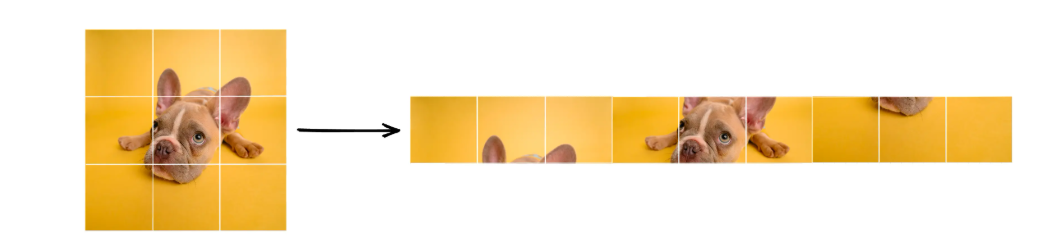
\includegraphics[width=\textwidth]{transformer_images/image_patch_embedding.png}
		\caption{iamge to patch}
		\label{fig:image to patch in vision transformer}
	\end{minipage}
	\hfill
	
\end{figure}


\subsection{شکل پچ ها:}

فرض کنید ابعاد تصویر ورودی ($H \times W \times C$) است. به‌عنوان مثال:


فرض کنیم اندازه تصویر ما $224 \times 224 \times 3$ باشد. یعنی طول و عرض تصویر به ترتیب 224 و سه کانال رنگی داشته باشد.
\[
H = 224, \quad W = 224, \quad C = 3
\]




\begin{figure}[h]
	\centering
	\begin{minipage}[b]{0.9\textwidth}
		\centering
		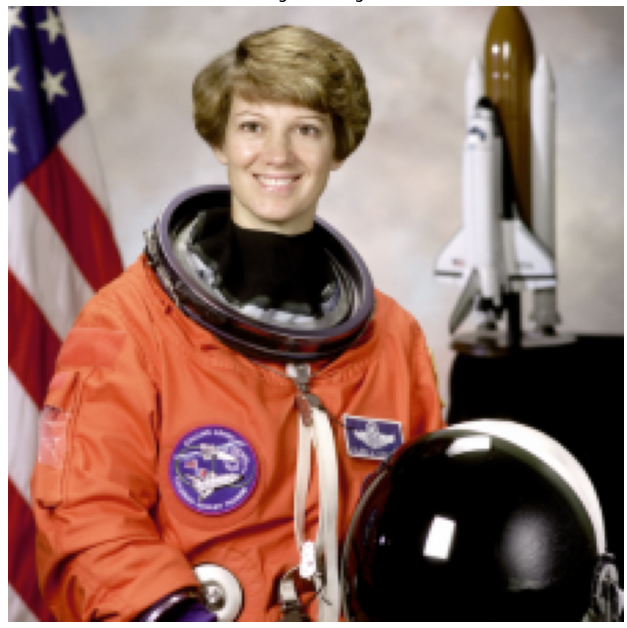
\includegraphics[width=\textwidth]{transformer_images/space_original_image.png}
		\caption{original Image}
		\label{fig:Original Image}
	\end{minipage}
	\hfill
	
\end{figure}


حال اگر اندازهٔ هر پچ ($P \times P$) باشد (مثلاً $16 \times 16$)، تصویر به‌صورت یک جدول مشبک از پچ‌های کوچک تقسیم می‌شود.

به هر پچ می‌توان مانند یک «کاشی» از تصویر نگاه کرد:
پچ اول: مختصات (0 تا 15 در ارتفاع) و (0 تا 15 در عرض)،
پچ دوم: مختصات (0 تا 15 در ارتفاع) و (16 تا 31 در عرض)،
و به همین ترتیب تا کل تصویر پوشش داده شود.



\begin{figure}[h]
	\centering
	\begin{minipage}[b]{0.9\textwidth}
		\centering
		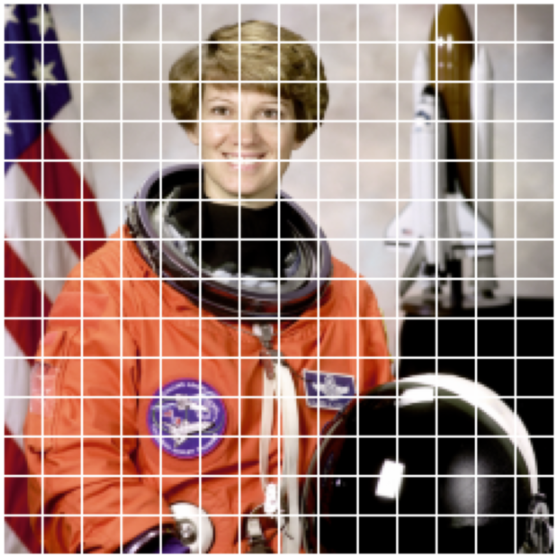
\includegraphics[width=\textwidth]{transformer_images/space_patch_iamge.png}
		\caption{patch Image}
		\label{fig:Patch Image}
	\end{minipage}
	\hfill
	
\end{figure}

\subsection{تعداد پچ ها:}

اگر پچ‌های ما بدون هم‌پوشانی باشند، ابعاد پچ دقیقاً باید بر ابعاد تصویر بخش‌پذیر باشد.


تعداد پچ‌ها افقی:
\[
\frac{W}{P}
\]
تعداد پچ‌ها عمودی:
\[
\frac{H}{P}
\]
در مجموع:
\[
\left(\frac{H}{P}\right) \times \left(\frac{W}{P}\right) = \frac{H}{P} \times \frac{W}{P}.
\]

برای مثال اگر:
\[
H = 224, \quad W = 224, \quad P = 16:
\]
\[
\frac{224}{16} = 14 \quad \Rightarrow \quad 14 \times 14 = 196 \quad \text{(تعداد پچ‌ها)}.
\]


